\section{Mechanical Design}\label{mec_sec}

This robot was designed and built using CAD (Computer Aided Design) and CAM
(Computer Aided Manufacturing) software. Moreover, extensive testing was done
to validate the current project.

Most of our robot parts were CNC machined and made out of 7075 aluminium and
high density polyoxymethylene (POM). The POM have some excellent prop- erties
such as high rigidity, good impact resistance, a non-stick characteristic and
beng a highly machinable material. In this way, some parts of the robots, like
the plunger stopping body, are more suitable to be made out of POM than
aluminium. For example, the dribbler arm is a pivot-rotating mechanism, and
using POM eliminates the need for a bearing within the assembly.

%\begin{figure}[thpb]
%    \centering
%    \begin{subfigure}[b]{0.49 \textwidth}
%        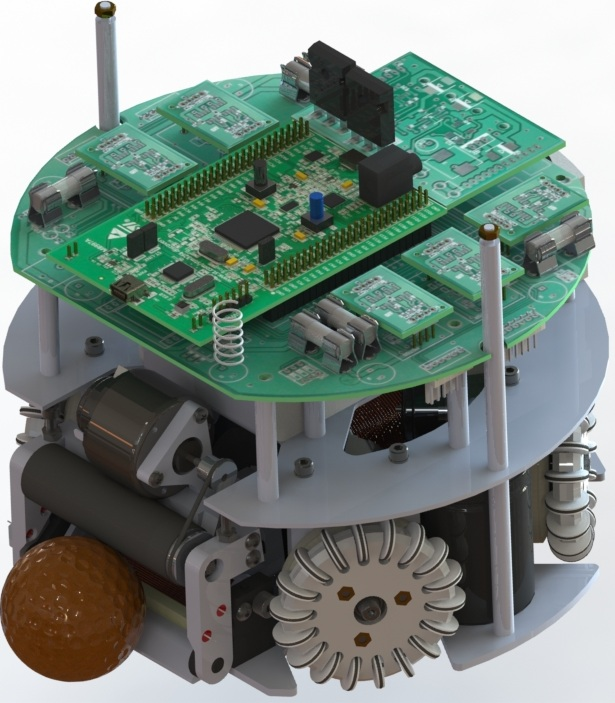
\includegraphics[width=\linewidth]{modeladof2}
%        \caption{3D model view.}
%        \label{fig:modelado}
%    \end{subfigure}
%    \begin{subfigure}[b]{0.49 \linewidth}
%        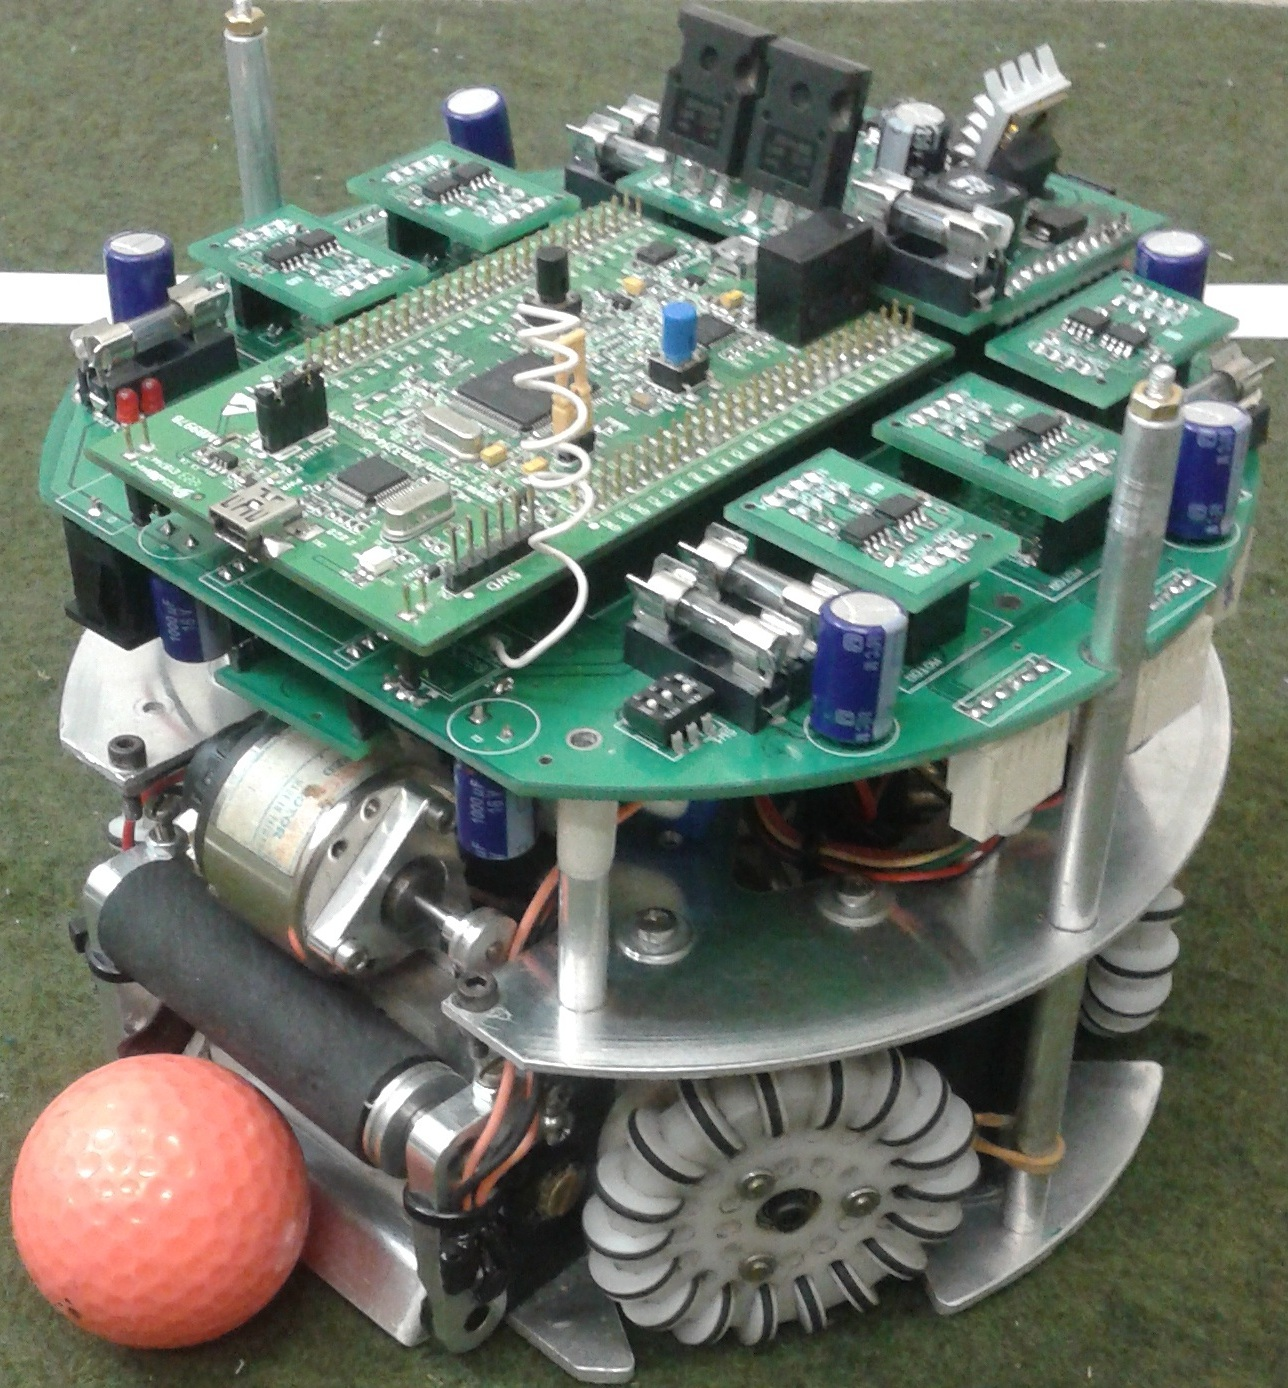
\includegraphics[width=\linewidth]{realf2}
%        \caption{Real robot view.}
%        \label{fig:real}
%    }
%    \end{subfigure}
%\end{figure}

\begin{figure}[ht]
    \subfloat[]{%
        \label{fig:modelado}
        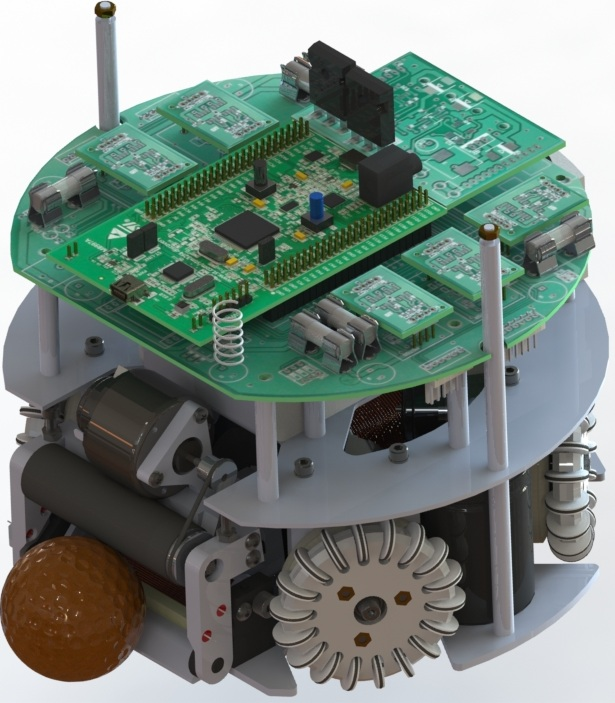
\includegraphics[width=0.47\linewidth]{modeladof2}
    }
    \subfloat[]{%
        \label{fig:real}
        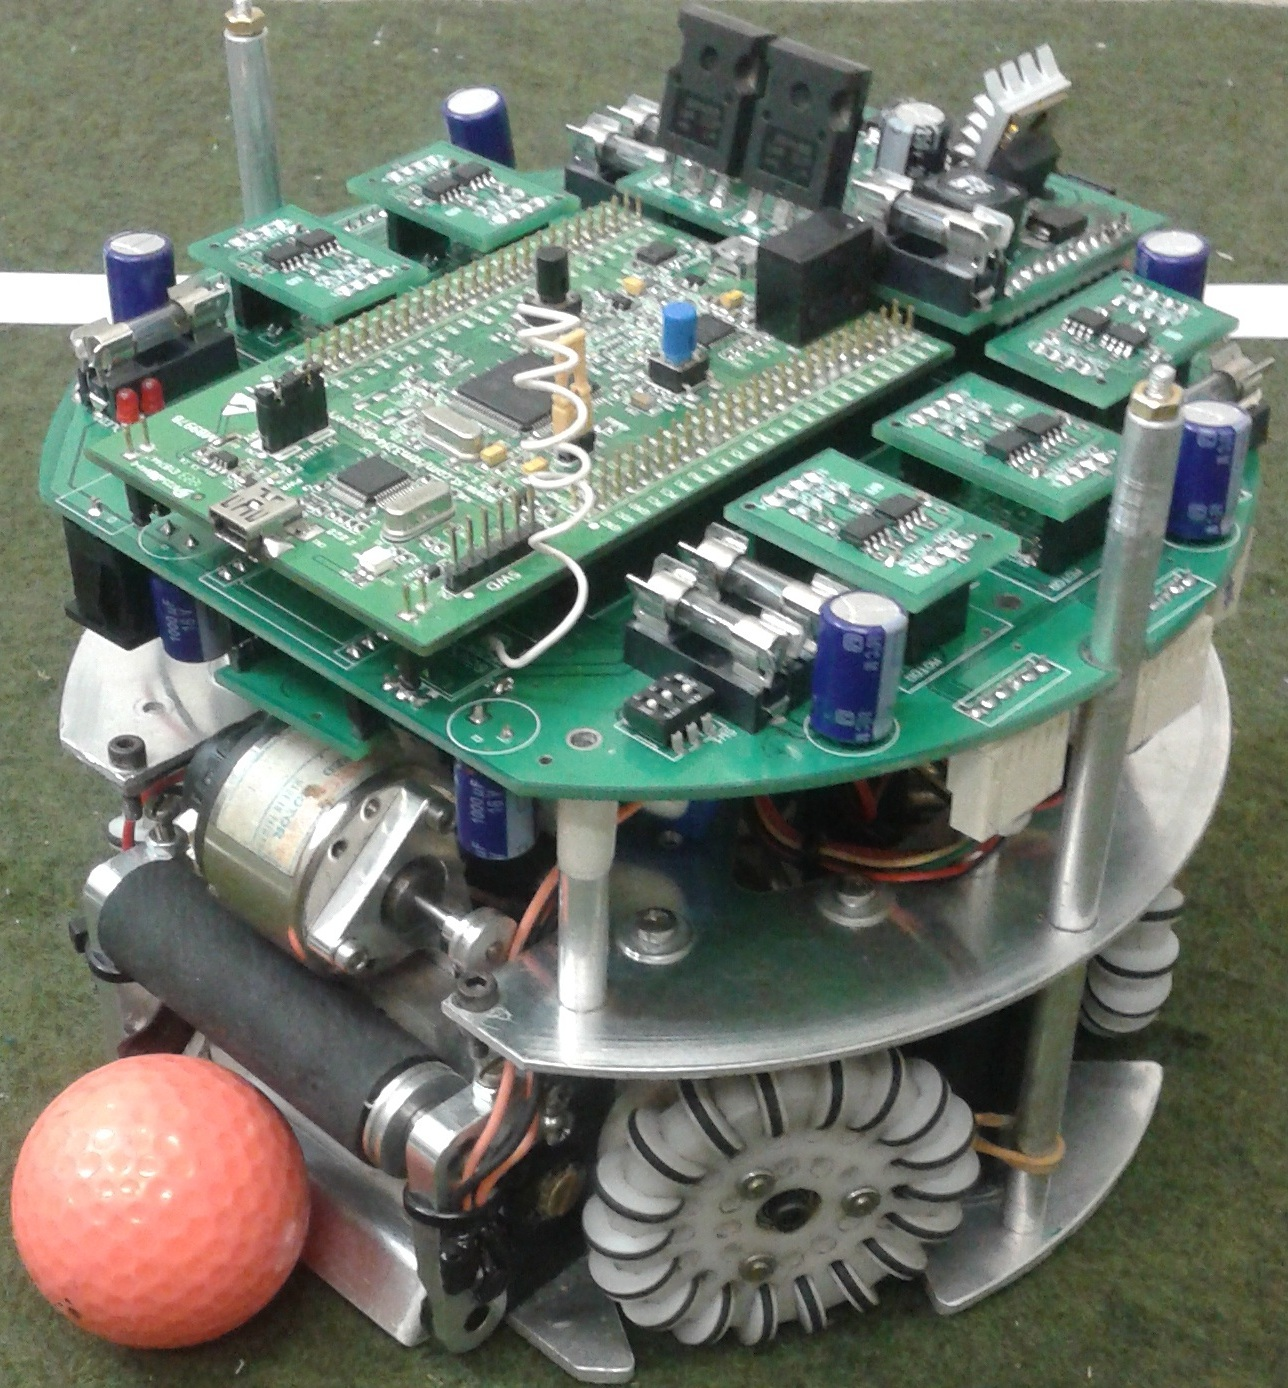
\includegraphics[width=0.47\linewidth]{realf2}
    }
    \label{fig:real_and_model}
    \caption{3D model~\ref{fig:modelado} and real robot~\ref{fig:real} views.}
\end{figure}


\subsection{Dimensional Constraints}
In compliance with the SSL rules, the height of the robot is 149 mm and the
maximum projection of the robot on the ground is 180 mm.

\begin{figure}[ht]
    \centering
    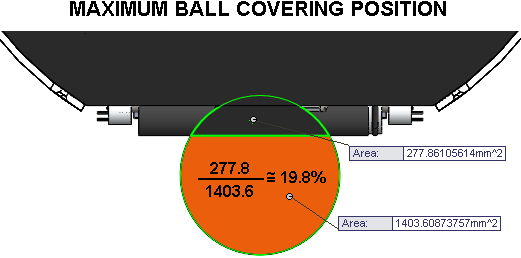
\includegraphics[width=\linewidth]{20-80_rule}
    \caption{Maximun covered area of the ball.}
    \label{fig:20-80_rule}
\end{figure}

Using CAD software we were able to measure the percentage of the ball area that
was covered by the robot. The maximum percentage of ball coverage found was
19,8\%, in accordance to the 20/80 rule of the league. The height of the
dribbler cylinder is also adjustable, so we are able to find the optimum point
for the best ball control.


\subsection{Transmission System}

A system of internal gears was made to transfer the power of the motors to the
wheels. This system has several advantages compared to traditional gear
meshing, such as avoiding debris entering the motors, creating a cavity to
apply grease for lubrication of gears and an overall smaller size.

However there are some difficulties in the manufacturing of this part, mainly
due to the small size of the teeth needed to mesh with standard motor gear (the
motor being used is the Hsiang Neng DC brushed motor type HN-GH35GMB). At this
motor the distance between two consecutive teeth is less than 1 mm, thus it was
not feasible to machine the internal gear. So it was decided for 3D printing in
ABS plastic as the manufacturing process.

The traditional fused filament deposition method for 3D printing, in geometries
smaller than the filament itself, create cavernous structures that weaken the
piece. Applying the stereolithography 3D printing process (when a laser beam
cure a liquid resin layer by layer), we manage to achieve a higher resolution.
This way we can precisely print the teeth profile, avoiding failures due to
empty spots and achieving a more solid and precise component.


\subsection{Chip Kick}

The chip kick is based on a flat solenoid, which is mounted in a slot at the
chassis (close to the ground). When activated the core of mild steel is
accelerated against the rear of the chip, which revolves around its axis and
makes the ball rise. Due to the limited space, complex construction and
details, we also have chosen the 3D printing as the manufacturing process.


\begin{figure}[tbph]
    \centering
    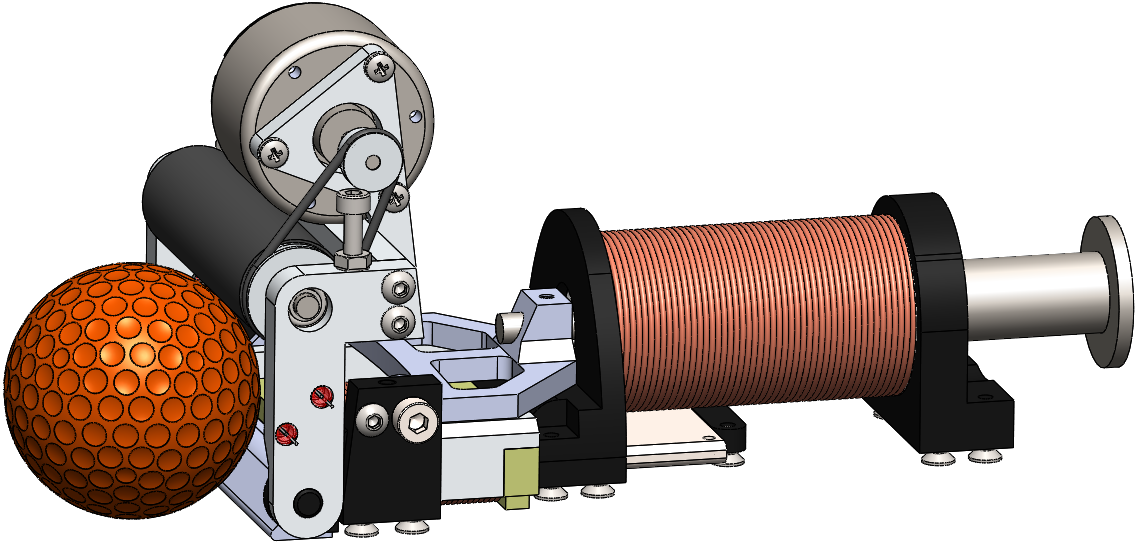
\includegraphics[width=\linewidth]{fechado}
    \caption{Dribbler, chipper and kicker assembly.}
    \label{fig:fechado}

    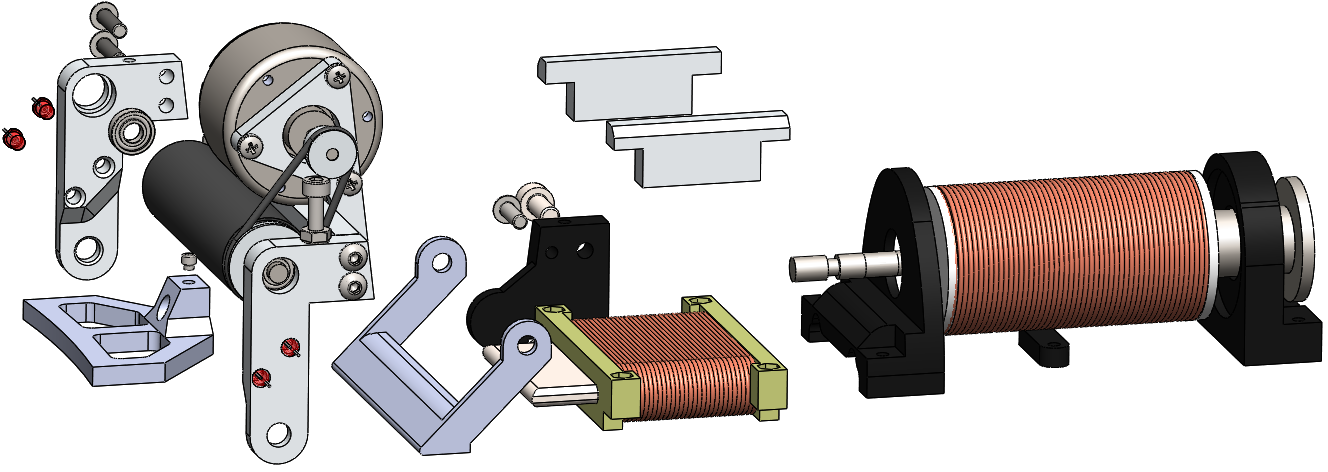
\includegraphics[width=\linewidth]{explodida}
    \caption{Exploded view.}
    \label{fig:explodida}
\end{figure}

The flat solenoid is assembled in a way that works as a guide rail for the kick
plunger as well. We are using rubber bands to pull back the chipper and kicker
plungers, keeping the mechanism simple. The final dribbling/kicking mechanism
is a very neat assembly and can be easily adapted for any other chassis.

% vim: tw=79 et sw=4 ts=4 filetype=tex
